%-------------------------------------------------------------------------------
\section{Introduction}
\label{s:intro}
%-------------------------------------------------------------------------------

Many microservices contend with varying load as well as being \textit{latency
critical} (LC), meaning they have strict SLOs that guarantee uptime and caps on
latency. However, when developers want to run microservices, scheduling systems
like AWS ec2 or Kubernetes required them to give a fixed amount of resources the
microservice needs, \ie{} a number of CPUs and an amount of memory~\cite{TODO}.
As a result, developers choose those requirements based on the expected peak
load, and the resources are rarely fully used~\cite{TODO}. 

Other tasks do not fall into this category: \textit{best effort} (BE) tasks such
as long-running map reduce jobs or background data analytics do not have an SLO.

Indeed, many modern scheduling systems separate the work they run into classes,
that include one class for LC tasks, which have resource requirements, and one
class for BE tasks, which don't. This includes distributed schedulers, \eg{}
Borg\cite{TODO} or Kubernetes\cite{TODO}, and single machine schedulers, \eg{}
Caladan\cite{TODO}. 

In an ideal world, BE tasks allows providers to get high utilization by
oversubscribing their machines without compromising any guarantees: Under high
load, microservice workloads run without impediment, but in low load BE tasks
run opportunistically and the servers maintain high utilization.

However, realizing high utilization and while enforcing strict isolation is
challenging. The scheduler needs to dynamically reallocate CPUs as the load
changes: it needs to maintain low latencies for LC requests by ensuring that
when the LC processes need resources they appear uncontended, while at the same
time using idle resources to run BE processes.

The current standard mechanism for isolating LC from BE processes is Linux's
\cgroups{}. Most modern containers rely on \cgroups{}; this includes all
Open Container Initiative (OCI) compliant containers, such as Docker,
Kubernetes, CRI-O, and containerd, because the OCI specification calls for use
of \cgroups{}. VMs, including Firecracker, AFaas, and KVM, also rely on
\cgroups{} to manage VMs when the number of vCPUs is oversubscribed.

The interface \cgroups{} exposes in order to specify the priority of processes
is based on weight: each workload is put into its own group, and each group is
assigned a weight in the range [1, 10000]. \cgroups{} specifies that each group
gets CPU time proportional to its weight as a share of the sum of weights of
runnable groups~\cite{TODO}.\footnote{Other operating systems use a similar
interface, for instance Windows exposes a number of shares.} For instance, if
two groups $cg1$ and $cg2$ have weights 200 and 300 respectively, when they are
both active their CPU time ratio should also be $2:3$. However, if $cg1$ has no
runnable threads, then $cg2$ would represent 100\% of the runnable weight and
get all the CPU time.

\begin{figure}[t]
    \centering
    \begin{subfigure}[b]{0.49\columnwidth}
        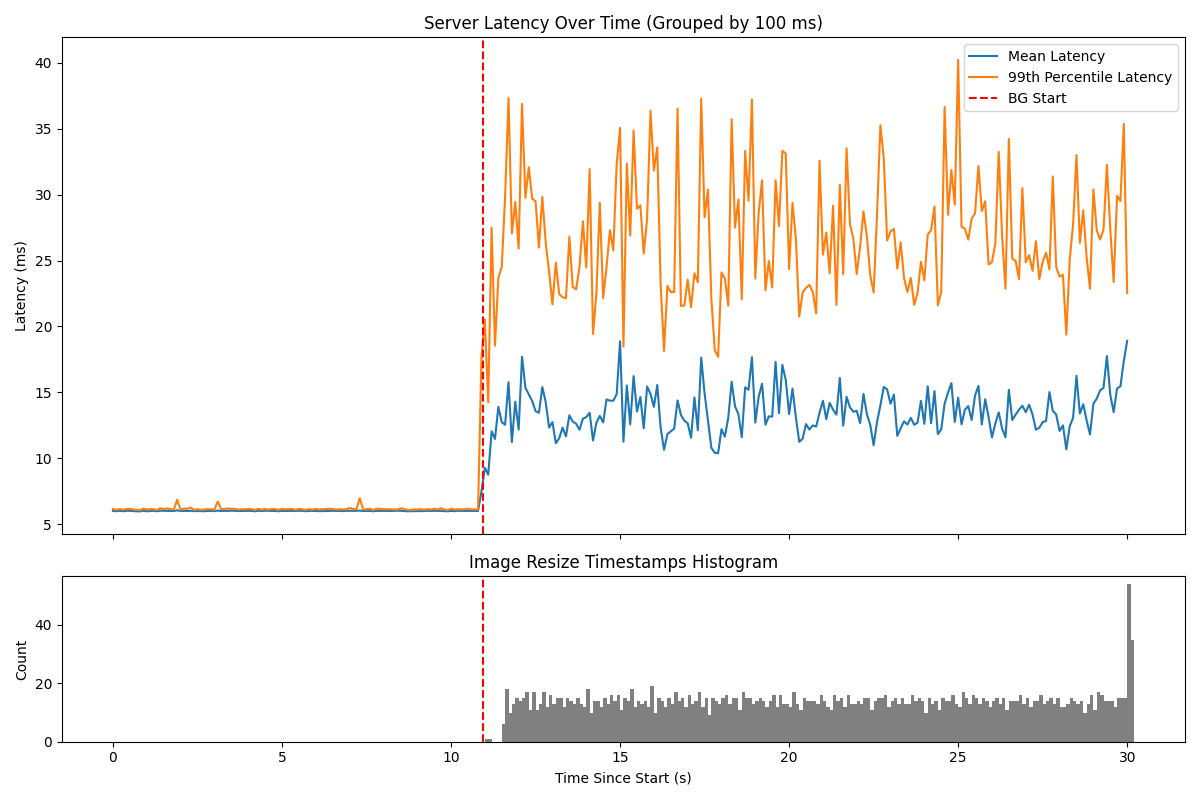
\includegraphics[width=\columnwidth]{graphs/unedited-weight-low-two.png}
        \caption{Low load stetting, utilization before starting the BE tasks is
        around 85\%}\label{fig:unedited-weight-low-two}
    \end{subfigure}
    \hspace{\fill}
    \begin{subfigure}[b]{0.49\columnwidth}
        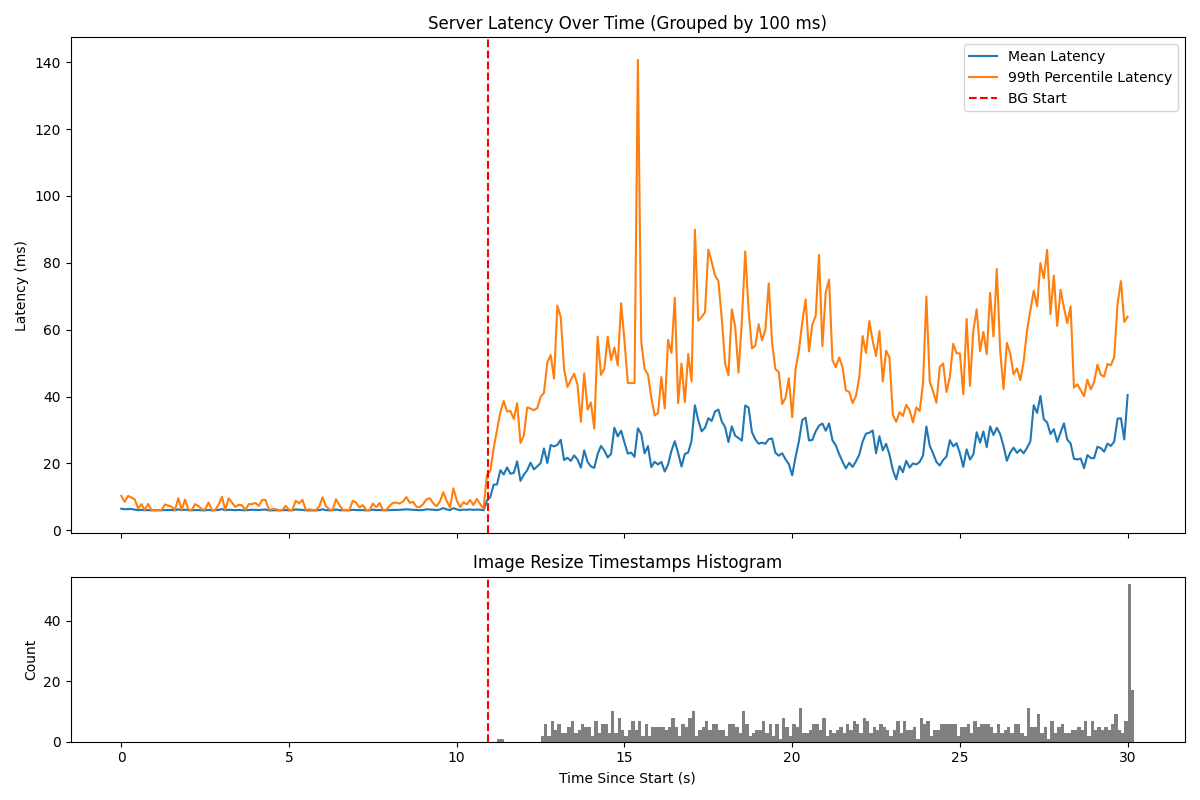
\includegraphics[width=\columnwidth]{graphs/unedited-weight-high-two.png}
        \caption{High load setting, utilization before starting the BE tasks is
        around 95\%}\label{fig:unedited-weight-high-two}
    \end{subfigure}
    \vspace{4pt}
    \caption{Latencies of the server and iteration counts of the background
    tasks in different load scenarios. Note the different y axis limits. The
    upper graphs show end-to-end request latencies, and the bottom graph is a
    histogram of completed iterations of the BE tasks}\label{fig:unedited-weight}
\end{figure}

In principle, the range of [1,10000] is large, and should allow for BE tasks to
have a negligible performance impact on LC tasks, even during high load.
However, we find that the presence of low weight (ie BE) tasks has a large
performance impact on a high-weight (ie LC) task. In an experiment, we run a
simple cpu-bound server and then start two BE workloads doing image resizing,
using two \cgroups{} groups, with weights 1 and 10000, to isolate the two.
\autoref{fig:unedited-weight} shows the increase in latencies of the LC server
at two different baseline utilization levels. We see that even in the lower
baseline utilization case, where the server alone uses 85\%, mean latencies
spike up from steady at around 6ms to as high as 20ms, and much higher for 99th
percentile latencies.

As we explore in \autoref{s:problem}, the main reason that this happens is that
Linux allows BE processes to run on one core, even while another core has a
queued and waiting LC process. This is an interface problem, not an
implementation bug: Linux's scheduler uses per-core runqueues, and as a result
the weights are only enforced on a runqeueue level.

Because of this, this paper argues that the split between LC and BE should be
categorical rather than ends of a weight spectrum, and that unfairness should be
the goal. We show that doing so enables Linux to isolate LC from BE:\ in the
same experiment, the increase in average latency when starting a BE workload
goes from $>$2x to 0, and the tail latency from $>$5x to 0. The contributions of
this paper are thus as follows: 
\begin{enumerate}
    \item the insight that weighted fair share breaks down with large weight
    splits because the weights are not enforced across cores; and that this
    dramatically affects end-to-end latencies
    \item showing that enforcing weights across core is prohibitively expensive,
    but categorical priorities are simpler to enforce, and that Linux does this
    well
    \item a patch to Linux that effectively creates a fully separated scheduling
    class that BE tasks can run in, which isolates LC workloads get from BE ones
    and minimizes the amount of added latency to do cross-core checks
\end{enumerate}
